\chapter{Domain Driven Design}

\section{Ubiquitous Language}

\begin{longtable}{|p{0.2\textwidth}|p{0.34\textwidth}|p{0.36\textwidth}|}
\hline
\textbf{Bezeichnung} & \textbf{Bedeutung} & \textbf{Begründung} \\
\hline
\code{Register} & 8-Bit-Speicherzelle im RAM des PIC-Mikrocontrollers & Zentraler Begriff der PIC-Hardware; wird in Datenblatt, Code und Kommunikation einheitlich verwendet. \\
\hline
\code{W} (Working Register) & Der Akkumulator-Register des PIC, über den alle arithmetischen Operationen laufen & Standardbezeichnung in der PIC-Architektur; im Code als \code{Register W} in der PIC-Klasse modelliert. \\
\hline
\code{Stack} & 8-Level-Hardware-Stack für Rücksprungadressen bei CALL/RETURN & Direkt aus der PIC-Hardware übernommen; gleichnamig im Code als Klasse \code{Stack}. \\
\hline
\code{Prescaler} & Vorteilerzähler, der die Eingangsfrequenz für Timer0 oder Watchdog herunterteilt & PIC-spezifischer Fachbegriff; im Code 1:1 als Klasse \code{Prescaler} mit \code{TMR0}/\code{WDT} Source modelliert. \\
\hline
\end{longtable}

\section{Repositories (1,5P)}

Die Applikation enthält \textbf{kein Repository} im DDD-Sinne. Begründung:

Ein Repository dient dem persistenten Speichern und Abrufen von Domain-Objekten (z.B. aus einer Datenbank). PICasso ist ein Echtzeit-Simulator, der den Zustand des Mikrocontrollers vollständig im Arbeitsspeicher hält. Es gibt keine Persistenzschicht: Programme werden bei jedem Start neu aus \code{.LST}-Dateien geladen, und der Simulationszustand wird nicht gespeichert. Die Domäne eines Hardware-Simulators erfordert keinen dauerhaften Speicher für Domain-Objekte -- der Zustand existiert nur während der Laufzeit, genau wie bei echter Hardware.

\section{Aggregates (1,5P)}

\textbf{Aggregate: \code{MemoryInterface}} als Aggregate Root über \code{Ram} und \code{Stack}.

\code{MemoryInterface} bildet eine transaktionale Grenze um den gesamten Speicherzustand: Es enthält \code{Ram} (2 Bänke $\times$ 80 Register) und \code{Stack} (8-Level). Alle Zugriffe auf den Speicher laufen über \code{MemoryInterface} -- direkter Zugriff auf \code{Ram} oder \code{Stack} von außen ist nicht vorgesehen. Dadurch stellt \code{MemoryInterface} die Konsistenz des Speicherzustands sicher (z.B. Bank-Switching, Registerspiegelung, Program Counter Synchronisation).

\begin{center}
    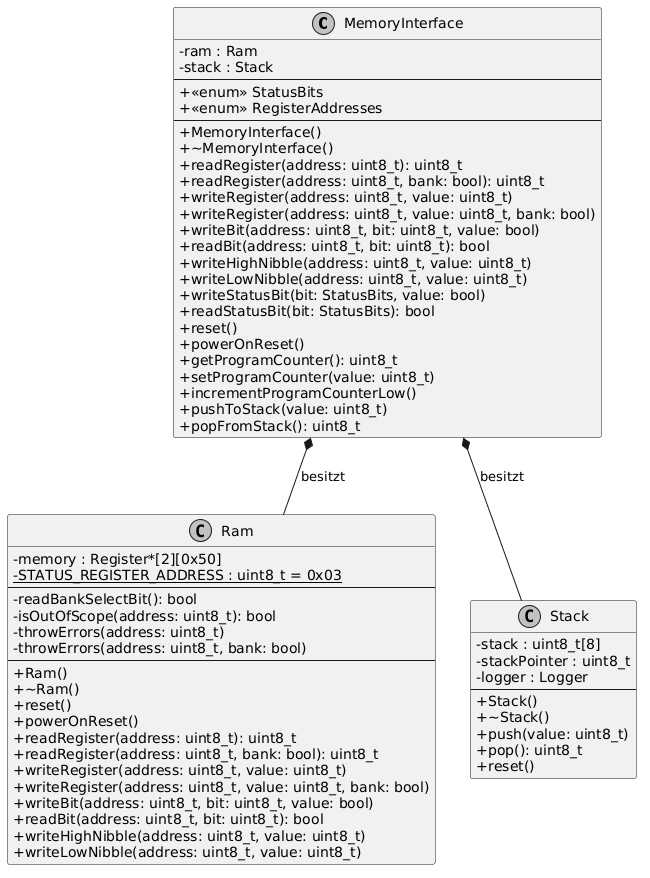
\includegraphics[width=0.9\textwidth]{UML/14.png}
\end{center}

\section{Entities (1,5P)}

\textbf{Entity: \code{PIC}}

Die \code{PIC}-Klasse repräsentiert eine konkrete Instanz eines PIC-Mikrocontrollers mit eigenem Zustand (RAM-Inhalt, W-Register-Wert, Program Counter, Simulationszeit). Zwei PIC-Instanzen mit identischem Aufbau unterscheiden sich durch ihren Zustand -- sie haben eine \textbf{Identität}, die über ihren Lebenszyklus bestehen bleibt. Der PIC durchläuft verschiedene Zustände (Power-On-Reset, laufende Simulation, Halt), behält aber seine Identität.

\begin{center}
    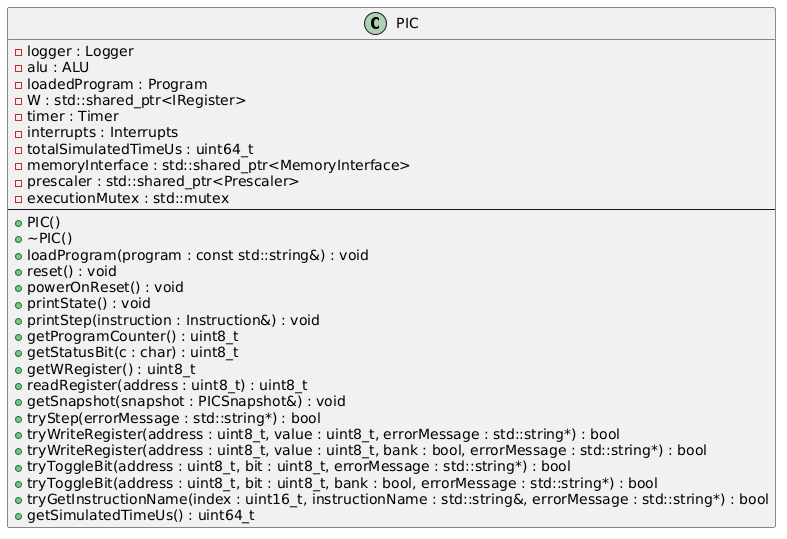
\includegraphics[width=0.9\textwidth]{UML/12.png}
\end{center}

\section{Value Objects (1,5P)}

\textbf{Value Object: \code{Bit}} (\code{header/memory/bit.hpp})

Die Klasse \code{Bit} ist ein klassisches Value Object:

\begin{itemize}
    \item \textbf{Immutability-Tendenz:} Ein Bit hat nur einen Wert (\code{true}/\code{false}), der seinen gesamten Zustand definiert.
    \item \textbf{Keine Identität:} Zwei Bits mit dem Wert \code{true} sind austauschbar -- es gibt keinen Grund, sie zu unterscheiden.
    \item \textbf{Gleichheit durch Wert:} Bits werden anhand ihres Wertes verglichen, nicht per Referenz.
\end{itemize}

Ebenso sind \code{Nibble}, \code{Byte} und \code{Register} Value Objects, da sie ausschließlich durch ihren gespeicherten Wert definiert werden.
\begin{center}
    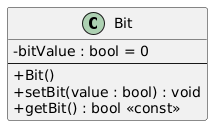
\includegraphics[width=0.5\textwidth]{UML/13.png}
\end{center}
